%\part{Der Bruhat-Tits-Baum für $\GL_2$}

%===========
\section{$p$-adische Zahlen}\label{sec_padisch}

Es sei $p$ eine Primzahl. Eine Zahl $n\in\NN$ lässt sich eindeutig
schreiben als
\[
n = \SUM{k}{i=0} a_i p^i
\]
mit $a_i\in\{0,\ldots,p-1\}$ und $k\geq 0$.

\BEM\label{def_ubertrag}
Wir rechnen mit Übertrag: Für $n=\sum a_i p^i$ und
$m=\sum b_i p^i$ ist
\begin{gather*}
m+n = \sum c_i p^i, \\
mn = \sum d_i p^i
\end{gather*}
mit
$c_i = \tilde{c}_i - \rho_i p$,
$d_i = \tilde{d}_i - \sigma_i p$,
wobei 
\[
\tilde{c}_i=a_i+b_i+\rho_{i-1},\quad
\tilde{d}_i=(\sum_{l=0}^i a_l b_{i-l})+\sigma_{i-1}
\]
und
$\rho_i = \left\{\begin{matrix}
1, & \tilde{c}_i \geq p \\
0, & \tilde{c}_i < p
\end{matrix}\right.,$
$\sigma_i=\max\{s\in\NN:sp\leq \tilde{d}_i\}$
ist.

\DB Die Menge
\[
\ZZ_p = \left\{
\SUM{\infty}{i=0} a_i p^i : a_i \in \{0,\ldots,p-1\}
\right\}
\]
wird mit $+$ und $\cdot$ wie in Definition \ref{def_ubertrag}
zu einem kommutativen Ring mit $1$. Er heißt
\emph{Ring der ganzen $p$-adischen Zahlen}.\index{p-adische Zahlen!Ring}\index{$\ZZ_p$ ($p$-adische Zahlen)}

\bew Wir zeigen, dass $(\ZZ_p,+)$ eine Gruppe ist:
\begin{align*}
-(\sum a_i p^i) &= (p-a_0) + (p-a_1-1) p + (p-a_2-1) p^2 + \ldots \\
&= (p-a_0) + \SUM{\infty}{i=1} (p-a_i-1) p^i.
\end{align*}
Es gibt also zu jedem Element ein additiv Inverses.

Die übrigen Ringeigenschaften sind klar.
\qed

\PROP\ \begin{enumerate}
\item Die Inklusion $\NN\subset \ZZ_p$ induziert eine Einbettung
$\iota:\ZZ\hookrightarrow \ZZ_p$.
\item $\ZZ_p$ ist nullteilfrei.
\end{enumerate}
\bew \begin{enumerate}
\item Für $n\in\ZZ$, $n<0$, setze $\iota(n):=-\iota(-n)$.
\item Es seien $a=\sum a_i p^i, b=\sum b_i p^i \in \ZZ_p\backslash\{0\}$ und
\[
i_a := \min\{i:a_i \neq 0\},\quad
i_b := \min\{i:b_i \neq 0\}.
\]
Für $ab=\sum d_i p^i$ ist dann $\tilde{d}_{i_a+i_b}=a_{i_a}b_{i_b}$
nicht durch $p$ teilbar, da $p$ prim ist.
Folglich ist auch $d_{i_a+i_b}=\tilde{d}_{i_a+i_b}-\sigma_i p$
nicht durch $p$ teilbar und insbesondere $\neq 0$.
Also ist $ab\neq 0$.
\qed
\end{enumerate}

\BEM Es sei
\[
\mm_p = \left\{
a=\SUM{\infty}{i=0} a_i p^i \in \ZZ_p : a_0\neq 0
\right\}.
\]
Dann gilt:
\begin{enumerate}
\item $\mm_p$ ist ein maximales Ideal.
\item $\ZZ_p/\mm_p \cong \ZZ/p\ZZ \cong \FF_p$.
\item $a\in \ZZ_p^\times$ genau dann, wenn $a\not\in\mm_p$.
\end{enumerate}
Insbesondere ist $\mm_p$ das einzige maximale Ideal in $\ZZ_p$,
d.h. $\ZZ_p$ ist ein lokaler Ring (vgl. Kapitel II.4 in 
Lang \cite{lang}).

\bew \begin{enumerate}
\item Offensichtlich ist $\mm_p$ ein Ideal. Die Maximalität
folgt aus Teil 2 oder 3.
\item Die Abbildung $a=\sum a_i p^i \mapsto \bar{a}_0\in \ZZ/p\ZZ$
ist ein surjektiver Ringhomomorphismus mit Kern $\mm_p$.
Der Homomorphiesatz liefert die Behauptung.
\item Es sei $a=\sum a_i p^i \in \ZZ_p\backslash \mm_p$, also
$a_0\neq 0$. Gesucht ist $b=\sum b_i p^i$ mit $ab=1$.
Definiere die $b_i$ induktiv: Da $p$ prim ist, kann man $b_0$ so 
wählen, dass $a_0 b_0 \equiv 1 \mod p$ gilt.
Hat man für $i\geq 1$ schon $b_0,\ldots,b_{i-1}$ gefunden, wähle
$b_i$ so, dass
\[
a_0 b_i + \SUM{i}{l=1} a_l b_{i-l} \equiv 0 \mod p
\]
gilt.
\qed
\end{enumerate}

\DB\
\begin{enumerate}
\item Der Quotientenkörper
\[
\QQ_p = \mathrm{Quot}(\ZZ_p)
\]
heißt \emph{Körper der $p$-adischen Zahlen}.\index{p-adische Zahlen!Körper}\index{$\QQ_p$ ($p$-adische Zahlen)}
\item Die Inklusion $\ZZ\hookrightarrow \ZZ_p$ induziert eine
Inklusion $\QQ\hookrightarrow \QQ_p$ (d.h. $\Char(\QQ_p)=0$).
\item Jedes $a\in \QQ_p^\times=\QQ_p\backslash\{0\}$ hat eine
eindeutige Darstellung
\[
a=\SUM{\infty}{i=i_a} a_i p^i
\]
mit $a_i\in\{0,\ldots,p-1\}$ und $i_a\in\ZZ$ minimal, so dass
$a_{i_a}\neq 0$.
\end{enumerate}
\textsc{Beweis von 3.:} Ist $a=\sum a_i p^i\in\ZZ_p\backslash\{0\}$,
so sei $i_a=\min\{i:a_i\neq 0\}$.
Dann ist $a=\SUM{\infty}{i=i_a} a_i p^i$ die gewünschte Darstellung.

Es ist $a=p^{i_a} u$ mit $u=\SUM{\infty}{i=0}a_{i+i_a} p^i\in\ZZ_p^\times$.
Nun sei $\frac{a}{b}\in\QQ_p$ mit $a,b\in\ZZ_p$, $b\neq 0$.
Schreibe $a=p^{i_a} u$ und $b=p^{i_b}v$ mit $i_a,i_b\in\NN$ und
$u,v\in\ZZ_p^\times$.
Es folgt
$\frac{a}{b}=p^{i_a-i_b} \ub{uv^{-1}}{\in\ZZ_p^\times}$,
wie gewünscht.
\qed

\DB\
\begin{enumerate}
\item Für $a=\SUM{\infty}{i=i_a}a_i p^i \in \QQ_p^\times$ sei
\begin{gather*}
\vv(a) := i_a,\\
|a| := p^{-i_a}.
\end{gather*}
\item Ist $a\in \ZZ$, so ist $\vv(a)=\max\{n:p^n|a\}$.
\item $a\in\ZZ_p\backslash\{0\}\ \lra\ \vv(a)\geq 0\ \lra\ |a|\leq 1$.
\item Setze $\vv(0):=\infty$, $|0|:=0$.
\item Für alle $a,b\in\QQ_p^\times$ gilt:
\begin{enumerate}
\item $\vv(ab)=\vv(a)+\vv(b)$ bzw. $|ab|=|a|\cdot |b|$.
\item $\vv(a+b)\geq\min\{\vv(a),\vv(b)\}$ bzw.
$|a+b|\leq\max\{|a|,|b|\}$.
\item Ist $\vv(a)\neq\vv(b)$, so ist $\vv(a+b)=\min\{\vv(a),\vv(b)\}$
bzw. $|a+b|=\max\{|a|,|b|\}$.
\item $\vv(a)=\vv(-a)$.
\end{enumerate}
\item $\vv:\QQ_p^\times \Ra \ZZ$ heißt \emph{$p$-adische Bewertung},
$|\cdot|:\QQ_p^\times \Ra \RR$ heißt \emph{$p$-adischer Betrag}.
\index{p-adische Bewertung}\index{p-adischer Betrag}\index{$\vv(a)$, $|a|$ ($p$-adische Bewertung)}
\end{enumerate}

\PROP\
\begin{enumerate}
\item $d(x,y):=|x-y|$ ist eine Metrik auf $\QQ_p$.
\item Jedes Dreieck in $\QQ_p$ ist gleichschenklig und die dritte
Seite ist höchstens so lang wie einer der gleichen Schenkel.
\end{enumerate}
\bew
\begin{enumerate}
\item Es gilt
\begin{gather*}
d(x,y)=0\ \lra\ x-y=0\ \lra\ x=y,\\
d(y,x)=|y-x|=|-(x-y)|=|-1|\cdot|x-y|=d(x,y)\\
\text{und}\\
d(x,z)=|x-z|=|(x-y)+(y-z)|\leq\max\{|x-y|,|y-z|\}\leq d(x,y)+d(x,z).
\end{gather*}
\item Folgt aus $|x-z|\leq \max\{|x-y|,|y-z|\}$.
\qed
\end{enumerate}

\PROP\ \begin{enumerate}
\item $\QQ_p$ ist vollständig.
\item $\QQ$ liegt dicht in $\QQ_p$.
\end{enumerate}
\bew \begin{enumerate}
\item Es sei $(a^{(n)})$ eine Cauchy-Folge in $\QQ_p$,
\[
a^{(n)} = \SUM{\infty}{i=i_a(n)} a_i^{(n)} p^i,
\]
mit $a_i^{(n)}\in\{0,\ldots,p-1\}$ und $i_a(n):=i_{a^{(n)}}$.
Es ist
\[
\vv(a^{(n)}) = i_a(n) \text{ und } |a^{(n)}|=p^{-i_a(n)}.
\]
Nun gilt
\[
|a^{(n)}-a^{(m)}| = p^{-\vv(n,m)}
\]
mit $\vv(n,m):=\min\{i:a_i^{(n)}\neq a_i^{(m)}\}$.
Folglich gibt es für jedes $i$ ein $n_0(i)$ mit $a^{(n)}_i=a^{(m)}_i$
für alle $n\geq n_0(i)$.
Da $a^{(n)}$ eine Cauchy-Folge ist, gibt es außerdem ein $i_0$
mit $a_i^{(n)}=0$ für $i<i_0$ und alle $n$.
Dann ist
\[
a = \SUM{\infty}{i=i_0} a_i^{(n_0(i))} \in \QQ_p
\]
der Grenzwert.
\item $\NN$ (und damit auch $\ZZ$) ist dicht in $\ZZ_p$, 
folglich ist auch $\QQ=\mathrm{Quot}(\ZZ)$ dicht in
$\QQ_p=\mathrm{Quot}(\ZZ_p)$.
\qed
\end{enumerate}

% ===============
\section{Der Baum für $\QQ_p$}\label{sec_baumQp}

\DEF Für $a\in \QQ_p$ und reelles $r>0$ sei
\[
\KU_r(a) := \{ b\in\QQ_p : |a-b|\leq r \}
\]
der \emph{Kreis}\index{Kreis!in $\QQ_p$}\index{$\KU_r(a)$ (Kreis in $\QQ_p$)}
um $a$ mit Radius $r$.

\BSP Kreise in $\QQ_p$.
\begin{enumerate}
\item $\KU_1(0)=\ZZ_p$.
\item $\KU_{1/p}(0)=\mm_p$.
\item $\KU_r(0)=\mm_p$ für alle $r$ mit $\frac{1}{p}\leq r < 1$.
\item $\KU_{1/p}(a)=\{ b\in\QQ_p:|b-a|<1 \}$, d.h. topologisch sind
offene und abgeschlossene Kreise in $\QQ_p$ nicht zu unterscheiden.
\end{enumerate}

\BEM Für Kreise $\KU_i=\KU_{r_i}(a_i)$, $i=1,2$, gilt:
\[
\KU_1\cap\KU_2=\emptyset\text{ oder }
\KU_1\subset \KU_2 \text{ oder }
\KU_2\subset \KU_1.
\]
Insbesondere ist $\KU_r(a)=\KU_r(b)$ für jedes $b\in\KU_r(a)$, d.h.
jeder Punkt in $\KU_r(a)$ ist Mittelpunkt.

\bew Es sei $a\in \KU_1\cap\KU_2$ und ohne Einschränkung
$r_1\leq r_2$. Dann gilt für $b\in \KU_1$:
\begin{align*}
d(b,a_2) &= |b-a_1+a_1-a+a-a_2| \\
&\leq \max\{\ub{|b-a_1|}{\leq r_1\leq r_2},
\ub{|a_1-a|}{\leq r_1\leq r_2},
\ub{|a-a_2|}{\leq r_2}\} \\
&\leq r_2.
\end{align*}
Also ist $b\in \KU_2$ und $\KU_1\subset \KU_2$.
\qed

Wir betrachten nun den Kreis $\KU=\KU_1(0)=\ZZ_p$.
Dieser Kreis enthält offensichtlich $\mm_p=\KU_{1/p}(0)$, also
die Elemente $a$ aus $\ZZ_p$ mit $a_0=0$.
\begin{center}
	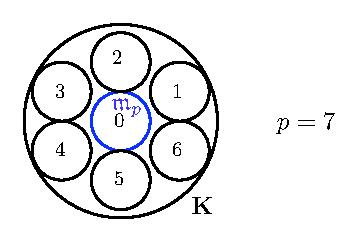
\includegraphics{grugraImages/kreisQp}
\end{center}
Für die übrigen Elemente von $\KU$ liegt $a_0\in\{1,\ldots,p-1\}$,
und $\KU$ enthält für jedes $a_0$ einen Kreis $\KU_{1/p}(i)$, dies
sind die Nebenklassen von $\mm_p$.
Die folgende Bemerkung verallgemeinert dies.

\BEM\ \label{bem_kreisQp}
\begin{enumerate}
\item Zu jedem Kreis $\KU=\KU_r(a)$ in $\QQ_p$ gibt es genau $p$
verschiedene maximale Kreise $\KU_1,\ldots,\KU_{p-1}$ mit
$\KU_i\subsetneq \KU$ für $i=1,\ldots,p-1$.
Es ist
\[
\KU_i = \KU_{r/p}(a+i p^{\lfloor\log_p(r)\rfloor}).
\]
\item Zu jedem Kreis $\KU=\KU_r(a)$ in $\QQ_p$ gibt es genau einen
minimalen Kreis $\KU'\supsetneq \KU$. Es ist
\[
\KU' = \KU_{rp}(a).
\]
\end{enumerate}

\DEF Es sei $T_p$ der Graph, der wie folgt definiert ist:
\begin{align*}
E(T_p) &= \{ \KU\subset\QQ_p : \KU \text{ ist Kreis} \}, \\
K(T_p) &= \{ (\KU,\KU') : \KU\subsetneq \KU' \text{ minimal oder }
\KU'\subsetneq \KU \text{ minimal} \},
\end{align*}
$\bar{(\KU,\KU')}=(\KU',\KU)$, $\ini(\KU,\KU')=\KU$ und
$\ter(\KU,\KU')=\KU'$.

Auf $T_p$ können wir eine kanonische Orientierung $K^+$ wählen,
indem wir aus jeder Kante $(\KU,\KU')$ den größeren der beiden Kreise
auswählen.\index{Orientierung}

\BEM $T_p$ ist ein Baum.

\bew $T_p$ ist zusammenhängend: Seien $\KU_i=\KU_{r_i}(a_i)$, $i=1,2$,
Kreise in $\QQ_p$. Ist $\KU_1\subset \KU_2$, so ist ohne Einschränkung
$a_1=a_2$ (denn jeder Punkt ist Mittelpunkt). Dann beschreibt
\[
\KU_1 \subset \KU_{r_1}p(a_1) \subset \ldots \subset
\KU_{r_1 p^k}(a_1)=\KU_2
\]
einen Weg in $T_p$.

$T_p$ enthält keine stachelfreien geschlossenen Wege: Wähle die
kanonische Orientierung $K^+$ auf $T_p$.
Es sei $w=(k_1,\ldots,k_n)$ ein stachelfreier Weg.
Beobachte, dass für $k_i\in K^-$ (d.h. $k_i=(\KU_i,\KU_{i+1})$
mit $\KU_i\subset \KU_{i+1}$) auch $k_{i+1},\ldots,k_n$ in $K^-$
liegen müssen (wegen Bemerkung \ref{bem_kreisQp}(2)).\\
Ist $w$ geschlossen, so gibt es ein $i$ mit $k_{i-1}\in\KU^+$ und
$k_i\in\KU^-$.
Folglich ist $\KU_{i-1}\subset \KU_i \supset \KU_{i+1}$, aber
$\KU_{i-1}\neq\KU_{i+1}$ (sonst gäbe es einen Stachel).
Also ist $\KU_{i-1}\cap \KU_{i+1}=\emptyset$. Wegen der obigen
Beobachtung ist $i$ eindeutig, also gilt
$\KU_0\subset \KU_{i-1}$ und $\KU_n\subset \KU_{i+1}$.
Und somit $\KU_0\neq \KU_n$, im Widerspruch dazu, dass $w$ geschlossen
sein soll. Somit kann $w$ nicht geschlossen sein.
\qed

\DEF Es sei $\GR$ ein Graph.
\begin{enumerate}
\item Ein \emph{Strahl}\index{Strahl} in $\GR$ ist ein Teilgraph,
der isomorph ist zu einer (in einer Richtung) unendlichen Kette.
\item Zwei Strahlen $R_1$ und $R_2$ heißen \emph{äquivalent}\index{Strahl!äquivalent},
wenn $R_1\cap R_2$ einen Strahl enthält.
\item Die Äquivalenzklassen von Strahlen heißen \emph{Enden}\index{Ende}.
\end{enumerate}
\begin{center}
	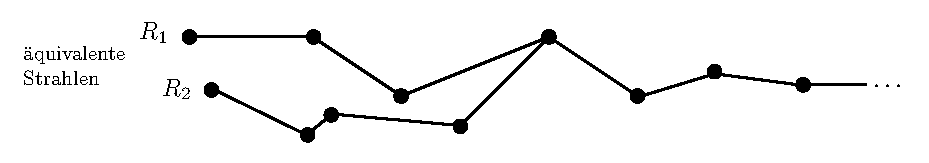
\includegraphics{grugraImages/R1R2}
\end{center}

\PROP Die Enden von $T_p$ entsprechen bijektiv den Punkten von
$\PP^1(\QQ_p)=\QQ_p\cup\{\infty\}$.\index{$\PP^1(\QQ_p)$ (projektiver Raum)}

\bew Suche eine Bijektion
\[
\phi:\{\text{Äquivalenzklassen von Strahlen in $T_p$}\}
\Ra \PP^1(\QQ_p).
\]
Es sei $R=(k_1,k_2,\ldots)$ ein Strahl in $T_p$.

Erster Fall: Alle $k_i\in K^+$. Setze $\phi(R):=\infty$.
Alle solchen Strahlen sind äquivalent.

Zweiter Fall: Fast alle $k_i\in K^-$ (d.h. alle ab einem $k_{i_0}$).
Es ist $\{a\}=\BCAP{}{i\geq i_0} \KU_i$.
Setze $\phi(R)=a$.

Man überzeugt sich leicht, dass $\phi$ wohldefiniert, surjektiv und
injektiv auf den Äquivalenzklassen von Strahlen ist.
\qed